\section{Experiments and Results}
\subsection{Experimental Setup}
The proposed framework was deployed on a real robotic baggage-handling platform. The platform consists of a collaborative robotic arm equipped with a hybrid suction--gripper end-effector, a conveyor belt operating at \revadd{493.2~mm/s}, and an Orbbec Gemini 435Le RGB-D camera with a resolution of $640\times400$ at 20~FPS. All algorithms were executed on an embedded AX650N processor. MSAM-Net inference, PX3C filtering, and CAOS stabilization were executed at every frame. \revadd{DKF state updates were executed at 5~Hz ($\Delta T=0.20~\mathrm{s}$), corresponding to a conveyor displacement of approximately 98.6~mm between updates.}

\begin{figure}[!t]
\centering
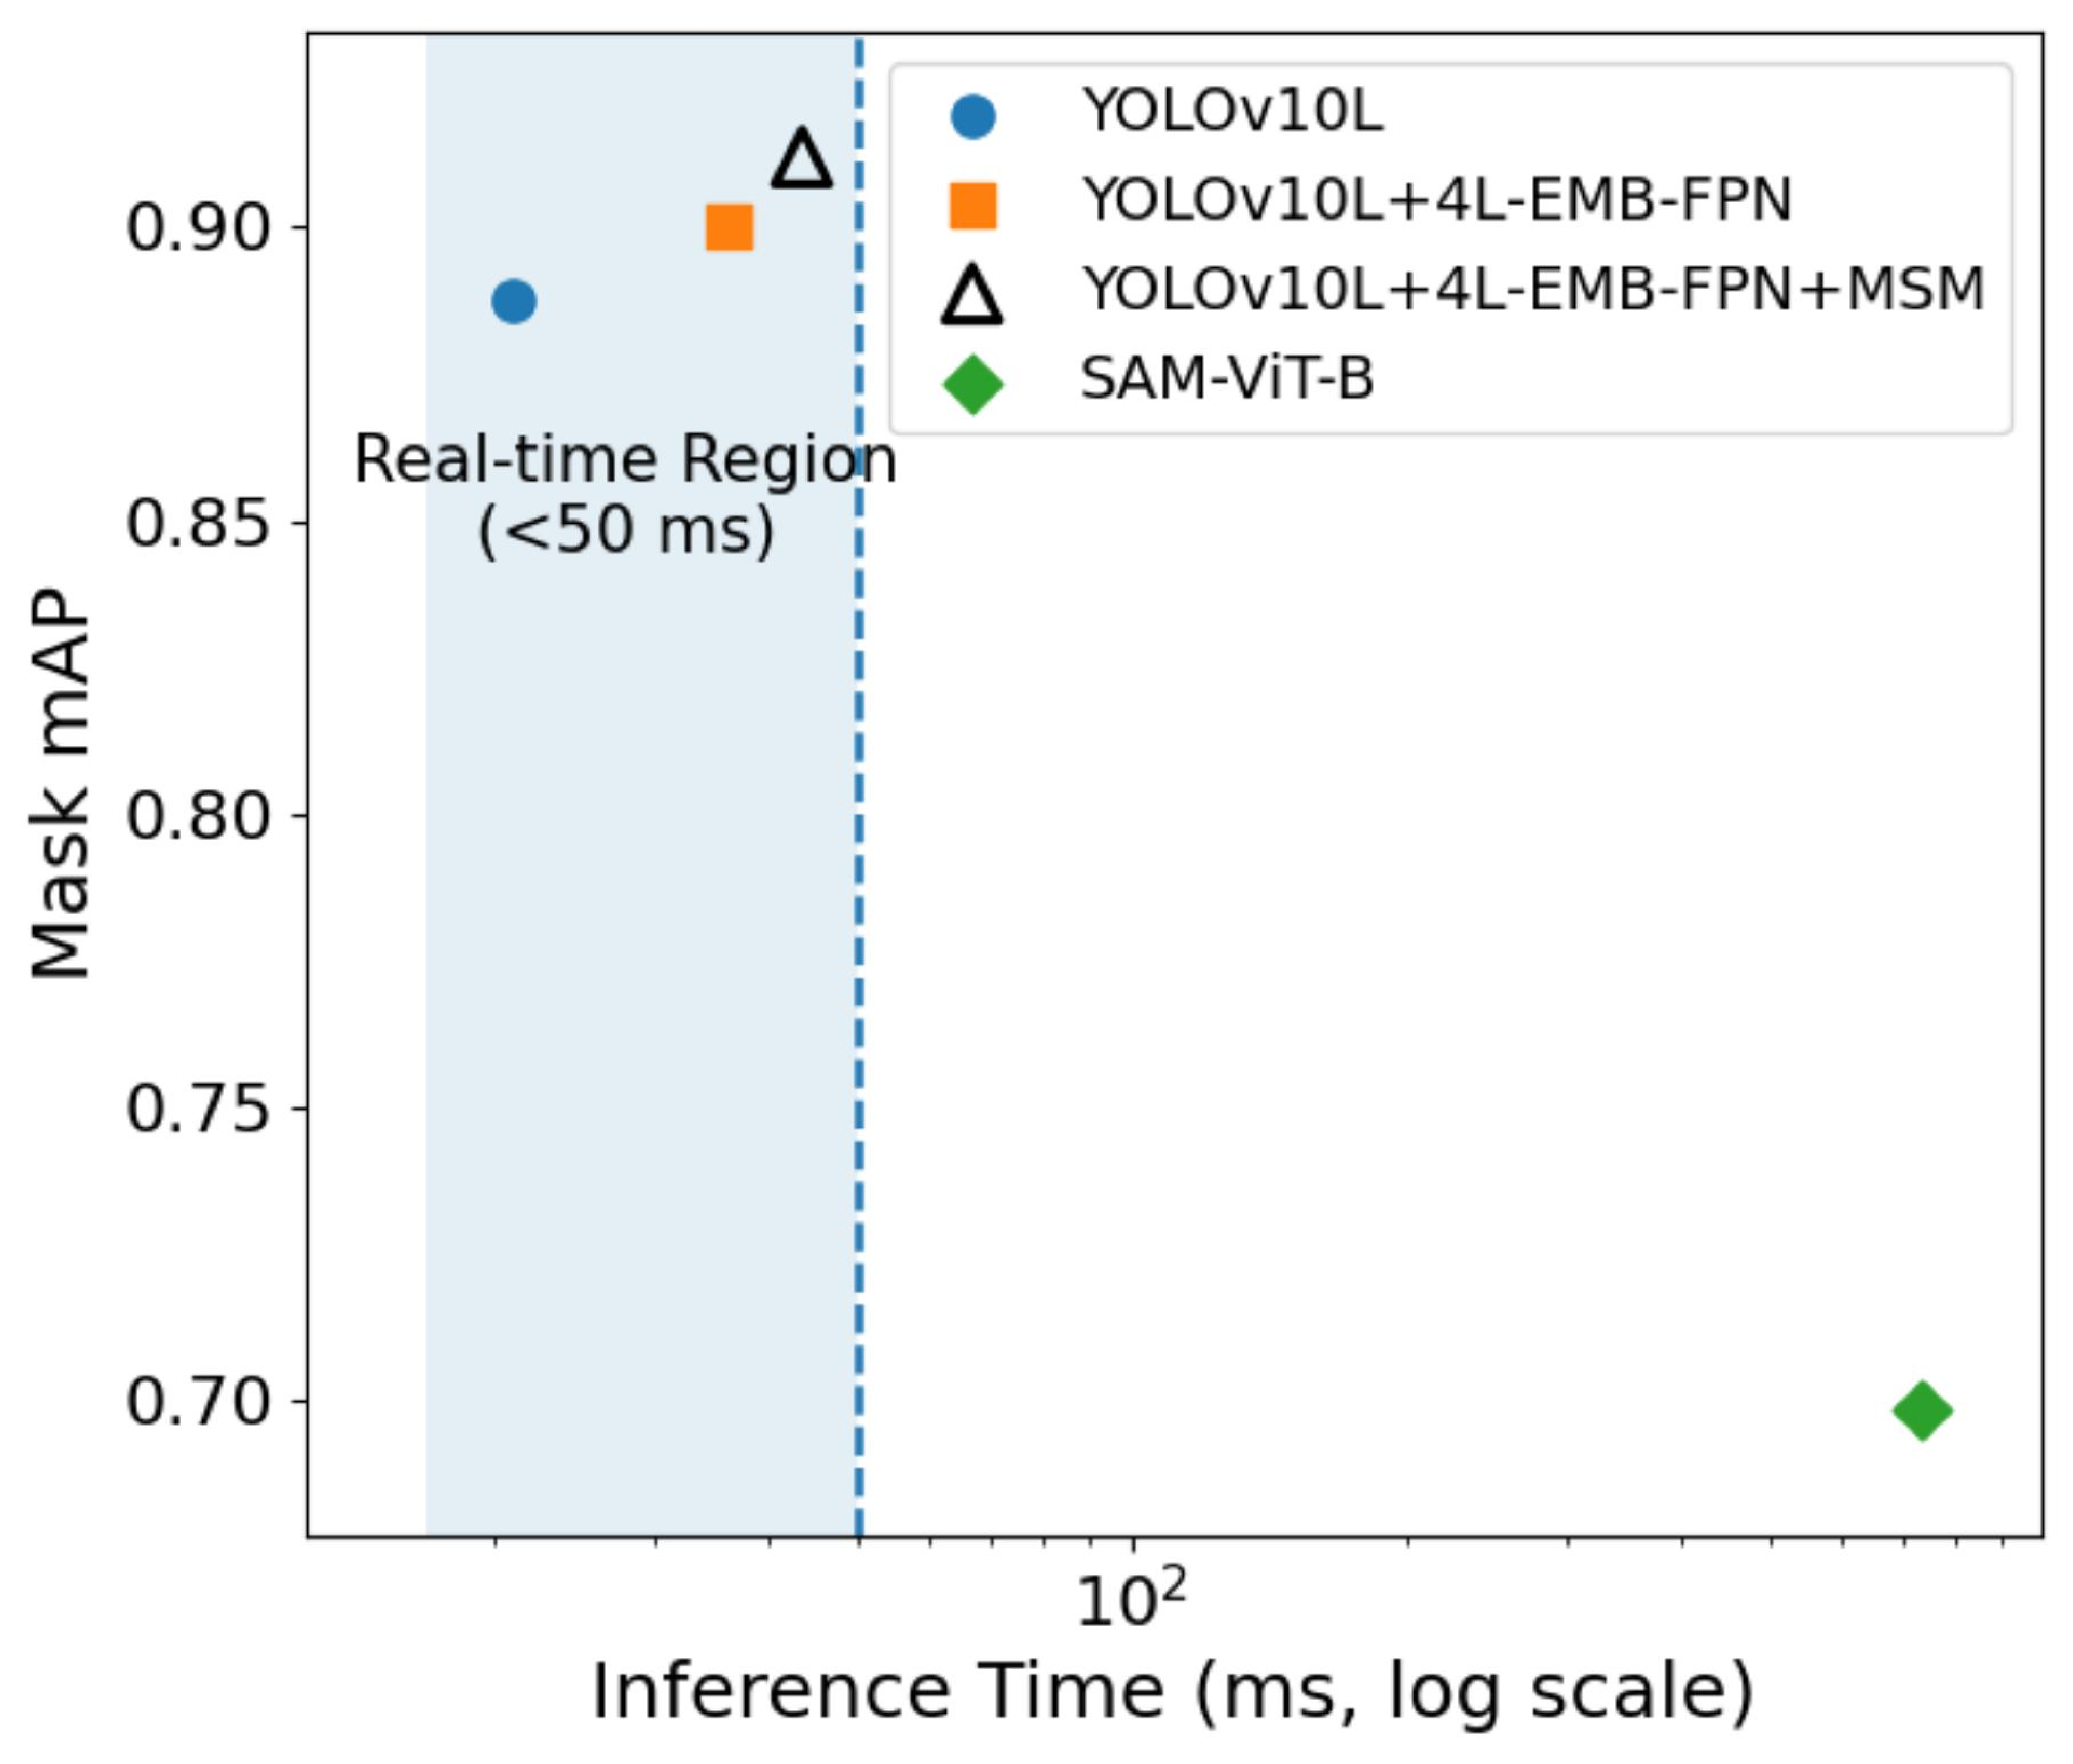
\includegraphics[width=\columnwidth]{figures/fig6.pdf}
\caption{Mask mAP versus inference time for different segmentation models.}
\label{fig:comparison_time}
\end{figure}

The baggage distribution was designed according to airport statistics collected from three airports across eight flights, including 515 items. Suitcases accounted for 94\% of the samples, soft bags for 5\%, and irregular objects for 1\%. More than 90\% of the samples contained strong tag interference. To simulate operational difficulty, random scenarios were generated, including single baggage placement (83\%), two-item contact (10\%), three-item stacking (2\%), and sidewall occlusion (5\%).

 \revadd{For 2D segmentation evaluation, SegData comprises SegData-train (49,359 images) and SegData-test (10,344 images), captured under different illumination, viewpoints, and distances. The splits were grouped by baggage instance, with no acquisition sequence shared between training and testing. Initial manual annotations were independently checked by a second annotator, and disagreements were corrected.} For 3D modeling evaluation, OBBData-test was constructed from 1,209 suitcase samples selected from SegData-test. \revadd{The ground-truth OBBs were manually checked and refined against the corresponding 3D point clouds, followed by independent review and correction of disagreements.} Suitcases were selected because they dominate the baggage distribution and provide stable centroid and yaw references, whereas soft bags are deformable and difficult to annotate consistently.

\revadd{Table~\ref{tab:geometry_parameters} summarizes the core parameters. PX3C used a 0.005~m voxel size, a 0.005~m RANSAC distance threshold with 500 hypotheses per frame, and a 5\% candidate-OBB trim fraction. Neighborhood filtering used a 0.03~m radius and at least three neighbors, with $\epsilon_{\mathrm{prot}}=0.005~\mathrm{m}$. CAOS used a 0.15~m clustering tolerance and a minimum cluster size of 500, with $\tau_{\mathrm{in}}=0.010~\mathrm{m}$, $(w_p,w_r,w_s)=(2.0,1.06,0.38)$, and $\eta=1.0$. The voxel, RANSAC, trimming, and conditional-filter settings followed experiment records; neighborhood and clustering settings were fixed implementation choices.}

\begin{table}[!t]
\color{red}
\centering
\caption{\revadd{Core parameters of Geometric Modeling, Motion Planning, and Active State Regulation.}}
\label{tab:geometry_parameters}
\footnotesize
\setlength{\tabcolsep}{5pt}
\renewcommand{\arraystretch}{1.08}
\begin{tabular}{@{}lc@{}}
\toprule
Parameter & Value \\
\midrule
\multicolumn{2}{@{}l}{\textit{PX3C}} \\
$\tau_{\mathrm{thin}}$ & $2.0$ \\
$\tau_{\mathrm{prot}}$ & $0.2$ \\
$\tau_{\mathrm{norm}}$ & $0.065$ \\
\midrule
\multicolumn{2}{@{}l}{\textit{CAOS}} \\
$\alpha_1,\alpha_2,\alpha_3$ & $0.43,\ 0.21,\ 0.36$ \\
$q_{\min}$ & $0.65$ \\
$\beta_{\max},k$ & $0.70,\ 2$ \\
\midrule
\multicolumn{2}{@{}l}{\textit{DKF, Motion Planning, and Active State Regulation}} \\
$\boldsymbol{Q}$ & $\mathrm{diag}([10^{-5},10^{-4},10^{-3}]_{\times3})$ \\
$\boldsymbol{R}$ & $\mathrm{diag}(2.5\!\times\!10^{-5},2.5\!\times\!10^{-5},10^{-4})~\mathrm{m}^2$ \\
$\lambda,\epsilon_{\mathrm{safe}}$ & $0.01,\ 0.01$ \\
$\tau_P$ & $4.0\times10^{-4}~\mathrm{m}^2$ \\
\bottomrule
\end{tabular}
\end{table}

\revadd{$\boldsymbol{Q}$ was initialized using the constant-acceleration model and adjusted through preliminary tracking experiments, whereas $\boldsymbol{R}$ was estimated from repeated static RGB-D measurements. Planning used $\Delta h=0.080~\mathrm{m}$, $\bar v=1.0~\mathrm{m/s}$, a Newton--Raphson tolerance of $10^{-3}~\mathrm{s}$, and $\alpha=1.2$ in \eqref{equ:estimate}. The interception height followed the required clearance, and synchronization references followed the conveyor speed and positioning tolerance: $v_{\mathrm{ref}}=0.4932~\mathrm{m/s}$ and $d_{\mathrm{ref}}=0.020~\mathrm{m}$. The remaining planning and active-regulation settings were selected through preliminary experiments. All settings were kept fixed during evaluation.}

\subsection{Segmentation Performance}
Three models were trained on SegData-train and evaluated on SegData-test: YOLOv10L, YOLOv10L with 4L-EMB-FPN, and YOLOv10L with both 4L-EMB-FPN and MSM, i.e., MSAM-Net. \revadd{The weights were set to $\lambda_{\text{box}}=7.5$, $\lambda_{\text{seg}}=7.5$, $\lambda_{\text{cls}}=0.5$, and $\lambda_{\text{dfl}}=1.5$, with $L_{\text{seg}}=L_{\text{mask}}+0.1L_{\mathrm{MSE}}$, where $L_{\text{mask}}$ denotes the cropped mask reconstruction loss and $L_{\mathrm{MSE}}$ is defined in \eqref{eq:mse}. These values were selected by grid search, with the loss-weight allocation guided by the official YOLO implementation.} Table~\ref{tab:seg} reports the quantitative segmentation results.

\begin{table}[!t]
\centering
\caption{Segmentation performance on SegData-test.}
\label{tab:seg}
\begin{tabular}{lcc}
\toprule
Method & Box mAP & Mask mAP \\
\midrule
YOLOv10L & 0.9185 & 0.8877 \\
+ 4L-EMB-FPN & 0.9417 & 0.9004 \\
+ MSM (MSAM-Net) & 0.9524 & 0.9120 \\
\bottomrule
\end{tabular}
\end{table}

The 4L-EMB-FPN improves mask mAP by 1.27\% compared with the YOLOv10L baseline, and the full MSAM-Net further increases the gain to 2.43\%. These results show that enhanced multi-scale aggregation and attention-guided mask refinement improve segmentation quality under tag and strap interference.

Inference latency on the AX650N processor is reported in Table~\ref{tab:latency}. MSAM-Net increases the inference time from \revadd{21.1~$\mathrm{ms}$} to \revadd{43.6~$\mathrm{ms}$}, but remains below the \revadd{50~$\mathrm{ms}$} real-time threshold required for 20~Hz conveyor-based manipulation. By comparison, SAM-ViT-B requires \revadd{733.6~$\mathrm{ms}$} per frame and is therefore unsuitable for embedded real-time deployment in this system \revadd{(as shown in Fig.~\ref{fig:comparison_time}).} SAM was evaluated without task-specific fine-tuning and achieved a mask mAP of 0.69. However, the comparison primarily demonstrates computational feasibility under industrial constraints.

\begin{table}[!t]
\centering
\caption{Inference time comparison on AX650N.}
\label{tab:latency}
\begin{tabular}{lc}
\toprule
Method & Inference time (ms) \\
\midrule
YOLOv10L & 21.1 \\
+ 4L-EMB-FPN & 36.1 \\
+ MSM (MSAM-Net) & 43.6 \\
SAM-ViT-B & 733.6 \\
\bottomrule
\end{tabular}
\end{table}

\begin{figure}[!t]
\centering
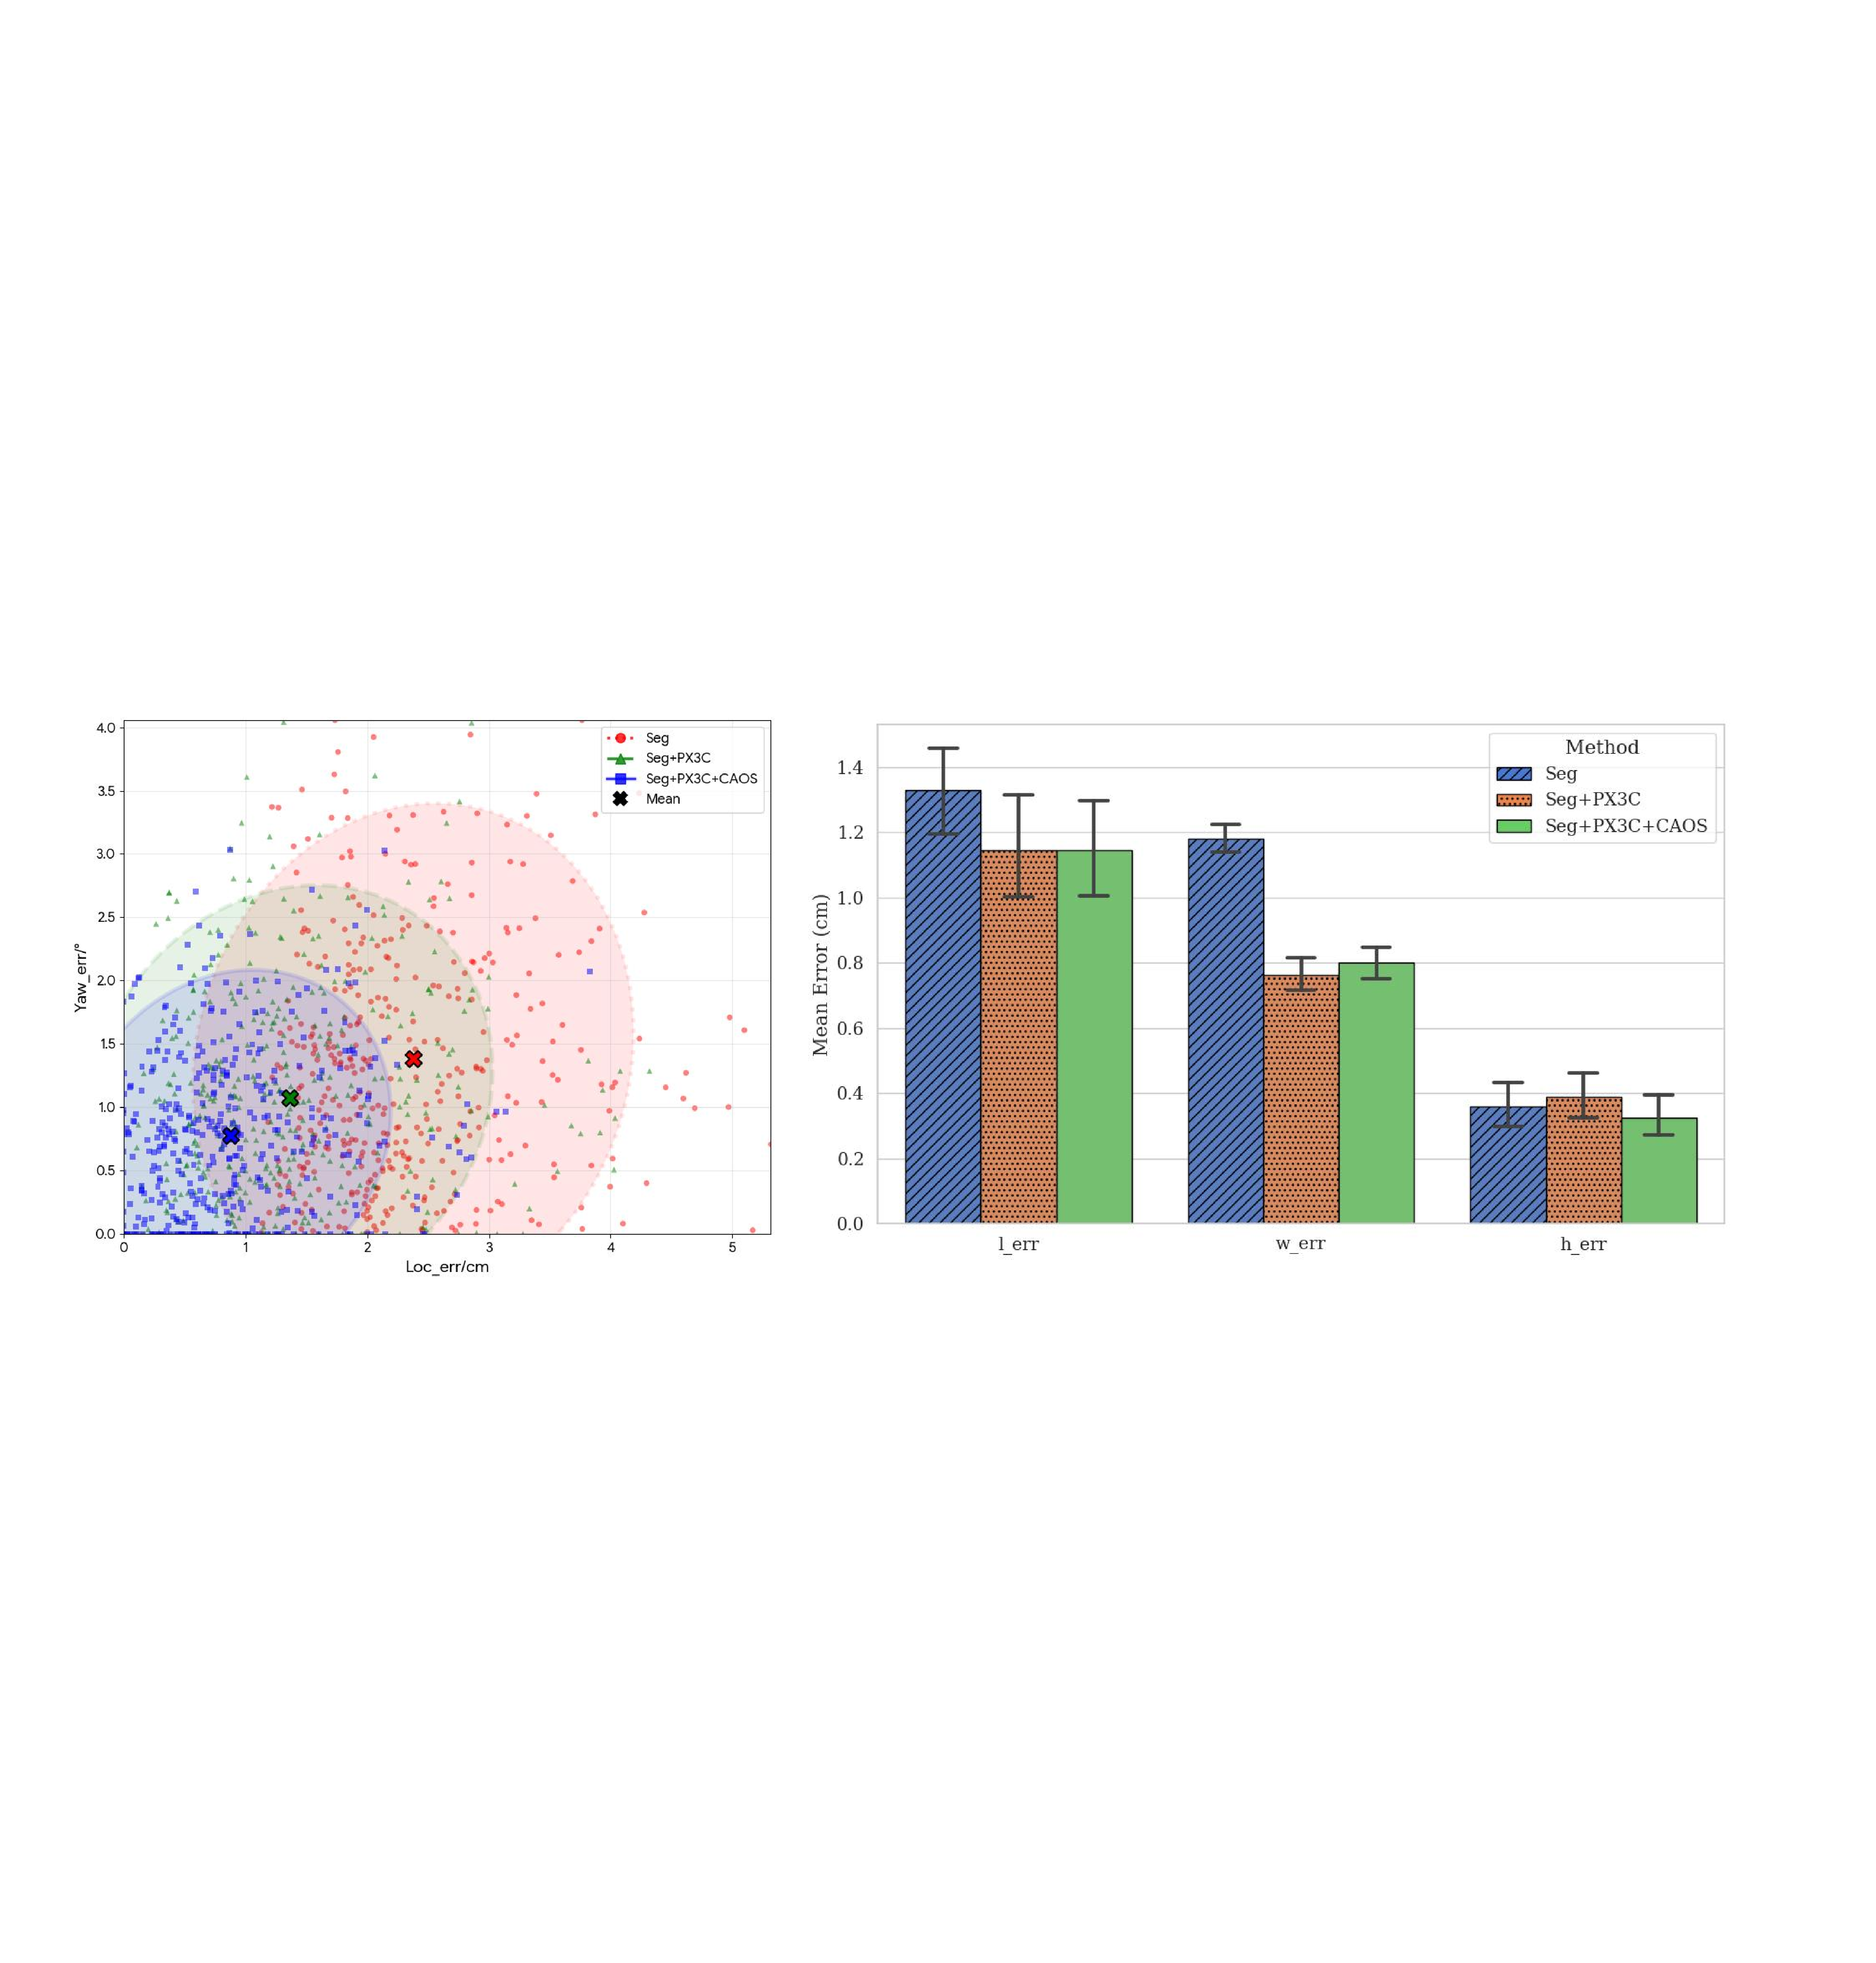
\includegraphics[width=\columnwidth]{figures/fig7_rev.pdf}
\caption{Comparison of pose and dimension estimation errors before and after PX3C and CAOS. Left: localization and yaw error distributions, with ellipses denoting 95\% confidence regions. Right: dimension estimation errors, with error bars indicating 95\% confidence intervals.}
\label{fig:estimation}
\end{figure}

\subsection{3D Modeling Accuracy}
To evaluate PX3C and CAOS, dimension and pose estimation errors were computed on OBBData-test. Dimension error was defined as the absolute error in length, width, and height. Pose error included centroid localization error and yaw error in the X--Y plane. Fig.~\ref{fig:estimation} compares pose and dimension estimation before and after PX3C and CAOS.

Compared with segmentation-only modeling, PX3C reduces the width estimation error by 35.5\%. The combined PX3C+CAOS pipeline further stabilizes the estimates. The length estimation error decreases by approximately 13.8\%, and the height estimation error reaches its minimum value of \revadd{0.33~$\mathrm{cm}$} when both modules are applied. The overall downward shift of the confidence intervals indicates consistent improvement.

The pose-error distributions are shown in Fig.~\ref{fig:estimation}. Each scatter point corresponds to one sample, and the ellipses denote 95\% confidence regions. Localization error decreases from \revadd{2.38~$\mathrm{cm}$} using segmentation-only modeling to \revadd{1.36~$\mathrm{cm}$} with PX3C and to \revadd{0.88~$\mathrm{cm}$} with CAOS. Yaw error decreases from $1.38^{\circ}$ to $0.78^{\circ}$. These results confirm that PX3C suppresses geometric outliers and CAOS reduces temporal fluctuations.

\begin{figure*}[!t]
\centering
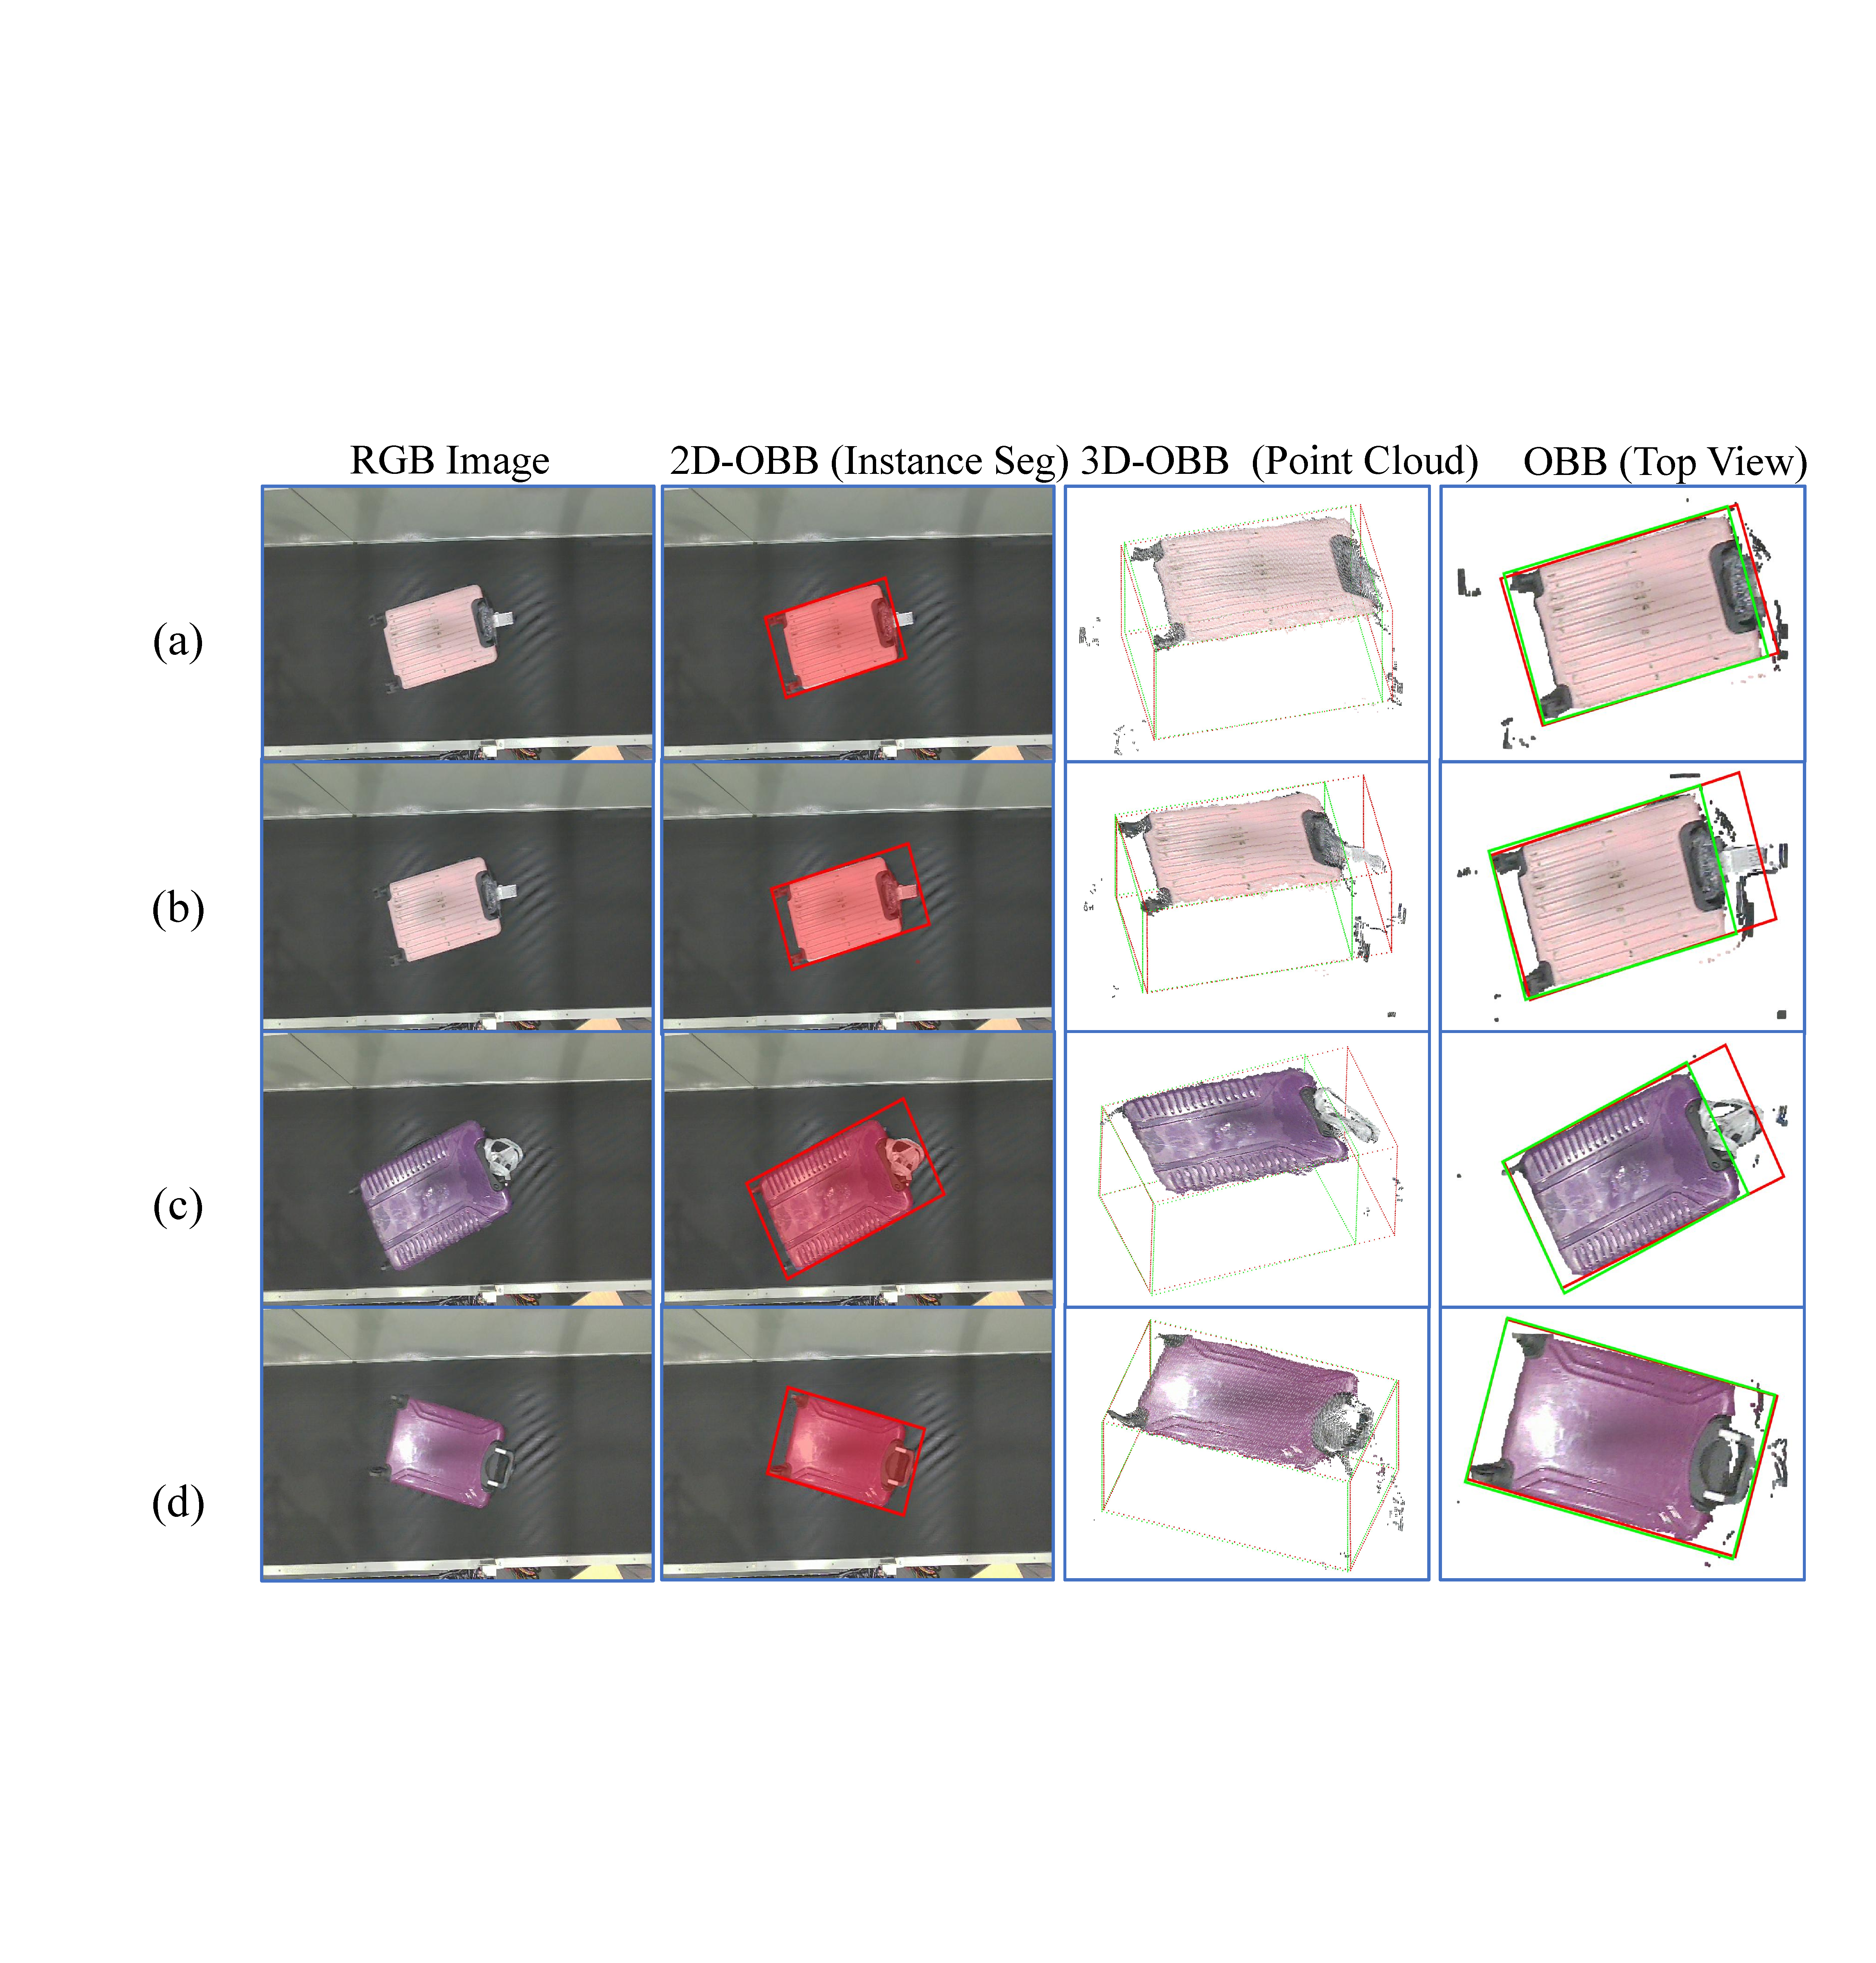
\includegraphics[width=\textwidth]{figures/fig9_rev.pdf}
\caption{Qualitative OBB comparison before and after PX3C filtering.}
\label{fig:represent}
\end{figure*}

Representative qualitative OBB comparisons are shown in Fig.~\ref{fig:represent}. Red boxes denote OBBs derived directly from segmentation, while green boxes denote refined OBBs after PX3C filtering. Flexible tags and ribbons are removed effectively, while rigid components such as handles and wheels are preserved. Temporal stabilization results are shown in Fig.~\ref{fig:temporal}, where CAOS reduces abrupt OBB fluctuations across consecutive frames caused by lighting variation, occlusion, and motion blur.

\begin{figure}[!t]
\centering
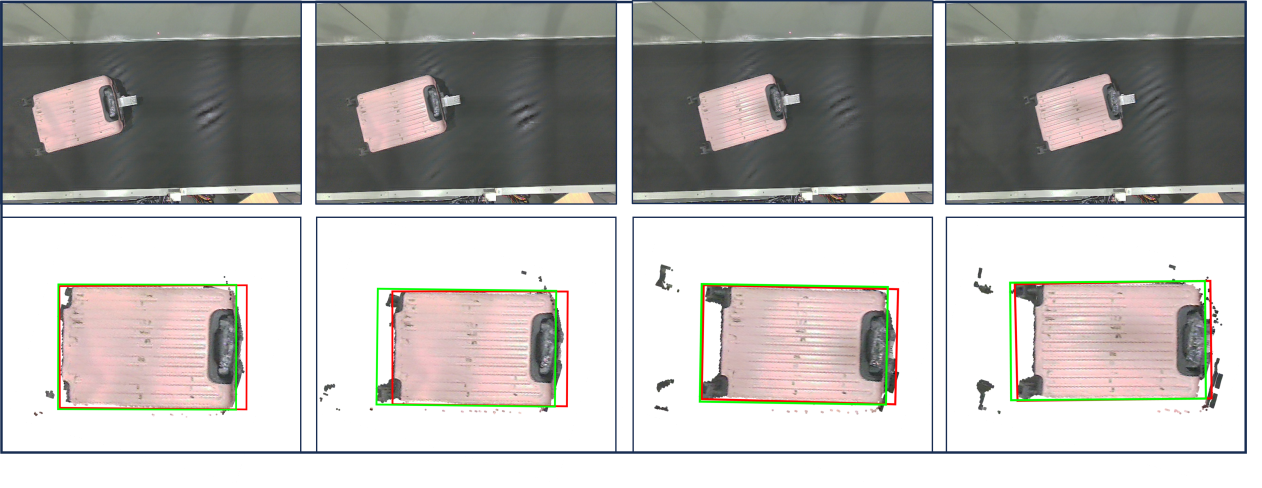
\includegraphics[width=\columnwidth]{figures/fig10.png}
\caption{OBB predictions across consecutive frames with CAOS stabilization.}
\label{fig:temporal}
\end{figure}



\subsection{System-Level Grasping Performance}
\revadd{Two metrics were used to evaluate system-level performance. General Success Rate (GSR) is the number of successful target grasps without dropping divided by all trials. Precision Success Rate (PSR) is the proportion of precise suitcase placements among successful suitcase grasps. We define precise placement as final placement with a position error below 2~$\mathrm{cm}$ and a yaw error below $5^{\circ}$, evaluated after the baggage has stabilized.} In multi-object scenarios, the highest object along the Z-axis was selected as the grasping target.

\revadd{Each of the five configurations was evaluated in 500 trials, for 2500 trials in total. Every configuration included 470 suitcase, 25 backpack, and 5 irregular-object trials, with the same scenario distribution: 83\% single-item placement, 10\% two-item contact, 2\% three-item stacking, and 5\% sidewall occlusion.} The snapshots are shown in Fig. \ref{fig:snapshot}. An ablation study was performed by incrementally integrating MSAM-Net, PX3C+CAOS, DKF+two-stage planning, and active state regulation. The results are summarized in Table~\ref{tab:ablation}. \revadd{For the full system, the short adjustment window on the moving conveyor limited each trial to at most one active reset. Relocation, renewed perception, replanning, and the subsequent gripper-based grasp belonged to the same trial and were counted once. A failed reset, failed subsequent grasp, or target leaving the robot workspace before grasp completion was counted as a failed trial. Intermediate reset placement was excluded from the final precision assessment.}

\begin{figure*}[!t]
\centering
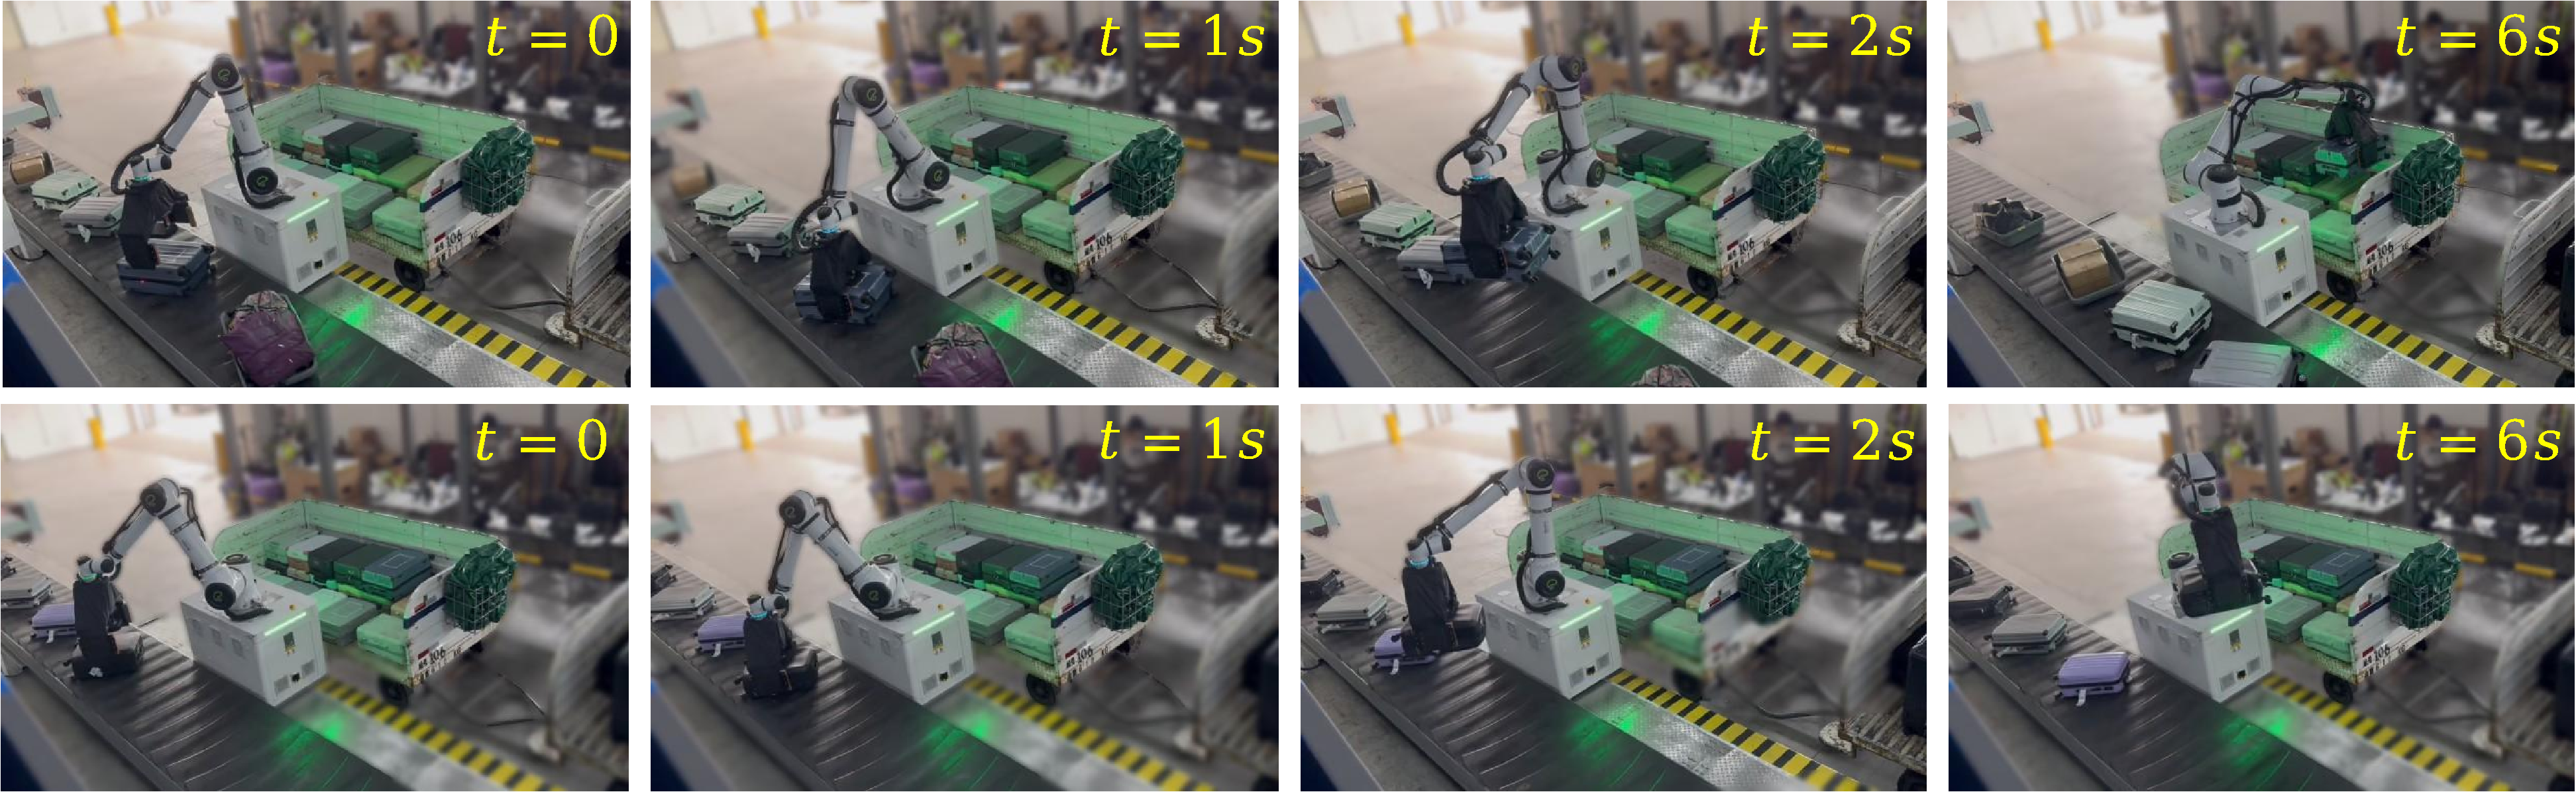
\includegraphics[width=\textwidth]{figures/fig8.pdf}
\caption{Snapshots of the dynamic grasping experiment. The proposed framework achieves robust dynamic grasping on a real conveyor belt in an industrial environment, overcoming the challenges of high-speed motion, cluttered scenes, and control uncertainty.}
\label{fig:snapshot}
\end{figure*}

\begin{table}[!t]
\centering
\caption{ \revadd{Ablation study with 500 trials per configuration.}}
\label{tab:ablation}
\setlength{\tabcolsep}{3pt}
\renewcommand{\arraystretch}{1.12}
\begin{tabular}{@{}>{\raggedright\arraybackslash}m{0.66\columnwidth}cc@{}}
\toprule
Method & GSR (\%) & PSR (\%) \\
\midrule
Baseline (YOLOv10L + PCL) & 93.6 & 62.1 \\
 \revadd{+ Instance segmentation (MSAM-Net)} & 95.2 & 69.6 \\
 \revadd{+ Geometric modeling (PX3C + CAOS)} & 95.6 & 83.8 \\
 \revadd{+ Predictive control (DKF + two-stage planning)} & 96.4 & 84.9 \\
+ Active State Regulation (full system) & 96.4 & 92.7 \\
\bottomrule
\end{tabular}
\end{table}

The GSR increases moderately from 93.6\% to 96.4\%, indicating that even the baseline system can lift many objects. In contrast, PSR increases substantially from 62.1\% to 92.7\%. \revadd{The gains of 2.8 and 30.6 percentage points, respectively, show that the framework primarily improves placement precision while maintaining a high grasp success rate.}

\revadd{In practical airport operations, baggage arrives with varying poses and stacking densities, making robust instance segmentation and pose estimation essential for reliable dynamic grasping. Successful lifting alone does not ensure that baggage can be placed according to a planned container layout. The PSR improvement indicates more accurate placement, which can help maintain the intended positions, orientations, and clearances between items. This provides a basis for tighter packing arrangements and higher packing density in subsequent aircraft baggage-loading deployment.}
